\section{Experiment}
\label{sec:exp}


\definecolor{lightgray}{gray}{.9}
\definecolor{lightblue}{RGB}{230,240,255}
\definecolor{lightgreen}{RGB}{230,255,230}
\definecolor{lightyellow}{RGB}{255,255,230}
\definecolor{lightred}{RGB}{255,230,230}
\definecolor{lightlightgray}{gray}{.95}
\definecolor{lightlightblue}{RGB}{240,245,255}
\definecolor{lightlightgreen}{RGB}{240,255,240}
\definecolor{lightlightyellow}{RGB}{255,255,240}
\definecolor{lightlightred}{RGB}{255,240,240}
\definecolor{lightlightlightgray}{gray}{.99}
\definecolor{lightlightlightblue}{RGB}{247,250,255}
\definecolor{lightlightlightgreen}{RGB}{247,255,247}
\definecolor{lightlightlightyellow}{RGB}{255,255,247}
\definecolor{lightlightlightred}{RGB}{255,247,247}


\begin{table*}[!t]
\begin{center}
    \setlength\tabcolsep{4pt} % 调整列间距，与第二个表格一致
    % \caption{}
    %
    \caption{\label{tab:main} Performance of \mymethod{} on the CogACT versus the other baselines in the SIMPLER environment. Settings vary by retained LLM layers (L) and visual tokens (T). \emph{Random Dropping} denotes a method involving the random retention of 112 visual tokens.}

    \vspace{5pt}
    \renewcommand{\arraystretch}{1.2} % 行高与第二个表格一致
    \resizebox{0.99\linewidth}{!}{%
        \begin{tabular}{l|c|c|ccccc|cccc} % 调整列定义，确保对齐方式一致
        \toprule\toprule % 双重顶部线
        \textbf{SIMPLER} & \textbf{Method} & \textbf{Training-free} & \textbf{PickCan} & \textbf{MoveNear} & \textbf{Drawer} & \textbf{DrawerApple} & \textbf{Average} & \textbf{FLOPs$\downarrow$} & \textbf{Speedup$\uparrow$} & \textbf{Params (B)} \\ 
        \midrule\midrule % 双重中间线
        \multirow{7}{*}{\begin{tabular}[l]{@{}l@{}}\textbf{Visual} \\ \textbf{Matching}\end{tabular}}  
          & \cellcolor{lightgray}CogACT & \cellcolor{lightgray}- & \cellcolor{lightgray}91.3\% & \cellcolor{lightgray}85.0\% & \cellcolor{lightgray}71.8\%&\cellcolor{lightgray} 50.9\% & \cellcolor{lightgray}74.8\%&\cellcolor{lightgray} 100.0\% &\cellcolor{lightgray} 1.00$\times$ & \cellcolor{lightgray}7.63 \\
          & \textcolor{gray!80}{\textbf{Random Dropping}} & \textcolor{green}{\ding{51}}& \textcolor{gray!80}{9.7\%} & \textcolor{gray!80}{20.4\%} & \textcolor{gray!80}{53.5\%} & \textcolor{gray!80}{0.0\%} & \textcolor{gray!80}{20.9\%} & \textcolor{gray!80}{58.5\%} & \textcolor{gray!80}{1.20$\times$} & \textcolor{gray!80}{7.63} \\
          & \textbf{FastV} & \textcolor{green}{\ding{51}}& 92.6\% & 81.4\% & 69.8\% & 52.4\% & 74.1\% & 42.0\% & 1.21$\times$ & 7.63 \\
          & \textbf{VLA-Cache} & \textcolor{green}{\ding{51}}& 92.0\% & 83.3\% & 70.5\% & 51.6\% & 74.4\% & 80.1\% & 1.38$\times$ & 7.63 \\
          & \cellcolor{lightyellow} \textbf{\mymethod{}} (L=28, T=112) 
            & \cellcolor{lightyellow}\textcolor{green}{\ding{51}}
            & \cellcolor{lightyellow}95.3\% & \cellcolor{lightyellow}83.3\% & \cellcolor{lightyellow}70.3\% & \cellcolor{lightyellow}56.5\% & \cellcolor{lightyellow}76.4\% 
            & \cellcolor{lightyellow}45.1\%
            & \cellcolor{lightyellow}1.59$\times$ & \cellcolor{lightyellow}5.87\\
          & \cellcolor{lightyellow} \textbf{\mymethod{}} (L=28, T=56) 
            & \cellcolor{lightyellow}\textcolor{green}{\ding{51}}
            & \cellcolor{lightyellow} 94.7\% & \cellcolor{lightyellow}82.4\% & \cellcolor{lightyellow}69.8\% & \cellcolor{lightyellow}55.4\% & \cellcolor{lightyellow}75.5\% 
            & \cellcolor{lightyellow}32.9\%
            & \cellcolor{lightyellow}1.71$\times$ & \cellcolor{lightyellow}5.87 \\
          & \cellcolor{lightyellow} \textbf{\mymethod{}} (L=22, T=112) 
            & \cellcolor{lightyellow}\textcolor{green}{\ding{51}}
            & \cellcolor{lightyellow}94.0\% & \cellcolor{lightyellow}82.1\% & \cellcolor{lightyellow}69.2\% & \cellcolor{lightyellow}54.6\% & \cellcolor{lightyellow}75.0\% 
            & \cellcolor{lightyellow} 38.2\%
            & \cellcolor{lightyellow}1.78$\times$ & \cellcolor{lightyellow}4.86 \\
          & \cellcolor{lightyellow} \textbf{\mymethod{}} (L=22, T=56) 
            & \cellcolor{lightyellow}\textcolor{green}{\ding{51}}
            & \cellcolor{lightyellow}93.3\% & \cellcolor{lightyellow}81.3\% & \cellcolor{lightyellow}68.2\% & \cellcolor{lightyellow}53.8\% & \cellcolor{lightyellow}74.2\% 
            & \cellcolor{lightyellow}28.9\% 
            & \cellcolor{lightyellow}1.93$\times$ & \cellcolor{lightyellow}4.86 \\
        \midrule
        \multirow{7}{*}{\begin{tabular}[l]{@{}l@{}} \textbf{Variant} \\ \textbf{Aggregation}\end{tabular}}  
          & \cellcolor{lightgray}CogACT & \cellcolor{lightgray}- & \cellcolor{lightgray}89.6\% & \cellcolor{lightgray}80.8\% & \cellcolor{lightgray}28.3\% & \cellcolor{lightgray}46.6\% & \cellcolor{lightgray}61.3\% & \cellcolor{lightgray}100.0\% & \cellcolor{lightgray}1.00$\times$ & \cellcolor{lightgray}7.63 \\
          & \textcolor{gray!80}{\textbf{Random Dropping}} & \textcolor{green}{\ding{51}}& \textcolor{gray!80}{4.0\%} & \textcolor{gray!80}{16.1\%} & \textcolor{gray!80}{15.6\%} & \textcolor{gray!80}{0.0\%} & \textcolor{gray!80}{8.9\%} & \textcolor{gray!80}{58.5\%} & \textcolor{gray!80}{1.20$\times$} & \textcolor{gray!80}{7.63} \\
          & \textbf{FastV} & \textcolor{green}{\ding{51}}& 91.4\% & 78.6\% & 27.6\% & 50.6\% & 62.1\% & 42.0\% & 1.19$\times$ & 7.63 \\
          & \textbf{VLA-Cache} & \textcolor{green}{\ding{51}}& 91.7\% & 79.3\% & 32.5\% & 45.8\% & 62.3\% & 82.6\% & 1.37$\times$ & 7.63 \\
          & \cellcolor{lightblue} \textbf{\mymethod{}}(L=28, T=112) 
            & \cellcolor{lightblue}\textcolor{green}{\ding{51}}
            & \cellcolor{lightblue}94.8\% & \cellcolor{lightblue}77.6\% & \cellcolor{lightblue}28.4\% & \cellcolor{lightblue} 51.9\% & \cellcolor{lightblue}63.2\% 
            & \cellcolor{lightblue}45.1\% 
            & \cellcolor{lightblue}1.57$\times$ & \cellcolor{lightblue}5.87 \\
          & \cellcolor{lightblue}  \textbf{\mymethod{}} (L=28, T=56) 
            & \cellcolor{lightblue}\textcolor{green}{\ding{51}}
            & \cellcolor{lightblue}94.4\% & \cellcolor{lightblue}77.2\% & \cellcolor{lightblue}27.6\% & \cellcolor{lightblue}51.3\% & \cellcolor{lightblue}62.6\% 
            & \cellcolor{lightblue}32.9\% 
            & \cellcolor{lightblue}1.69$\times$ & \cellcolor{lightblue}5.87 \\
          & \cellcolor{lightblue}\textbf{\mymethod{}} (L=22, T=112) 
            & \cellcolor{lightblue}\textcolor{green}{\ding{51}}
            & \cellcolor{lightblue}93.9\% & \cellcolor{lightblue}76.4\% & \cellcolor{lightblue}27.3\% & \cellcolor{lightblue}50.6\% & \cellcolor{lightblue}62.1\% 
            & \cellcolor{lightblue}38.2\% 
            & \cellcolor{lightblue}1.76$\times$ & \cellcolor{lightblue}4.86 \\
          & \cellcolor{lightblue}\textbf{\mymethod{}} (L=22, T=56) 
            & \cellcolor{lightblue}\textcolor{green}{\ding{51}}
            & \cellcolor{lightblue}93.2\% & \cellcolor{lightblue}75.8\% & \cellcolor{lightblue}26.9\% & \cellcolor{lightblue}49.2\% & \cellcolor{lightblue}61.2\% 
            & \cellcolor{lightblue}28.9\% 
            & \cellcolor{lightblue}1.91$\times$ & \cellcolor{lightblue}4.86 \\
        \bottomrule\bottomrule % 双重底部线
        \end{tabular}
    }
\end{center}
\vspace{-10pt}
\end{table*}




\subsection{Experimental Settings}
\label{sec:setting}
\noindent \textbf{Simulation Implementation Details}.
To assess our VLA model, we utilize the SIMPLER environment~\citep{li2024evaluating}, a simulation-based benchmark for table-top manipulation. SIMPLER is designed to closely emulate real-world dynamics for robots such as the Google Robot and WidowX, demonstrating robust alignment between simulation and real-world performance.
The VLA model in this setup takes 224$\times$224 RGB image observations and natural language task instructions (e.g., "Pick coke can") as input and outputs a sequence of actions in 7-DoF Cartesian space.
The SIMPLER supports two evaluation configurations: \emph{Visual Matching}, which prioritizes fidelity to real-world appearances, and \emph{Variant Aggregations}, which incorporates diverse conditions such as altered lighting, backgrounds, and surface textures. For the Google robot, SIMPLER provides both two evaluation settings, each featuring the same four tasks: 1) Pick coke can; 2) Move near; 3) Open/close drawer; and 4) Open top drawer and place apple. Success rate is used as the evaluation metric.
% \chuan{Briefly introduce the observation, such as image (in what resolution) and the task instruction, and action space which should be Cartesian Space Control.}

\noindent \textbf{Baselines}. Our primary experimental validation of \mymethod{} is performed on the \emph{CogACT}~\citep{li2024cogactfoundationalvisionlanguageactionmodel}, which integrates powerful vision encoders (DINOv2~\citep{oquab2023dinov2} and SigLIP~\citep{zhai2023sigmoid}), a Llama2-7B~\citep{touvron2023llama} language module for multimodal reasoning, and a Diffusion Transformer (DiT) for generating action trajectories. We benchmark against relevant baseline methodologies. These include a \emph{Random Dropping} approach, where 112 visual tokens are retained uniformly at random, to evaluate the benefits of our guided vision token pruning. We further compare with \emph{FastV}~\citep{chen2025image}, a notable approach focused on accelerating inference by pruning redundant visual tokens, and \emph{VLA-Cache}~\citep{xu2025vla}, which leverages temporal analysis to cache static tokens across timesteps.

\noindent \textbf{Implementation Details}.
For \mymethod{}, in addition to layer pruning, we further compressed the model parameters by adopting the PruneNet~\citep{prunenet} configuration for LLM compression. Specifically, we applied a sparsity of 25\% to the MLP layers of all Transformer blocks. For visual token pruning, we started from the 2nd Transformer layer with a ratio $\alpha$ = 50\% and $K_{key}$ = 4 for key task-critical tokens. Furthermore, the cache interval was set to 5. All experiments were conducted on NVIDIA A40 GPUs, and the inference time was measured as the average single-step inference duration. More details can be found in the supplementary material.



\subsection{Results on Simulation Environment}


\noindent \textbf{Main Results on SIMPLER}.
Table~\ref{tab:main} details the performance of our structured, entirely training-free pruning method in the SIMPLER environment. Our approach consistently excels across configurations retaining 22/28 layers and 56/112 visual tokens. For instance, pruning 10 layers with 112 tokens surpasses both CogACT and VLA-cache in success rate and inference speed. Remarkably, on the \emph{pick coke can} task, pruning 36\% of parameters paradoxically improved the success rate from 91.3\% to 94.0\%, highlighting significant parameter redundancy in the VLA model. Conversely, random token dropping to 112 tokens drastically reduces the average success rate to 20.9\%, affirming the superiority of our guided selection strategy. Furthermore, a 22-layer, 56-token setup achieved a 71.1\% reduction in FLOPs with merely a 0.6\% drop in average success rate, demonstrating exceptional efficiency. In comparision, approaches like FastV~\citep{chen2025image} (T = 56) show that solely optimizing visual tokens yields only a 1.21$\times$ speedup due to unaddressed memory bottlenecks, despite acceptable task performance.

% \noindent \textbf{Main Results on SIMPLER}.

\noindent \textbf{Efficiency Analysis}.
As demonstrated in Table~\ref{tab:main} and Figure~\ref{fig:compare}, our proposed method significantly outperforms previous baselines, achieving a 71.1\% reduction in FLOPs and a 1.93$\times$ speedup in inference time. In stark contrast, VLA-cache, when applied to the CogACT model, only reduces FLOPs by 19.9\% and achieves a mere 1.38$\times$ speedup. This disparity substantiates our prior analysis: VLA-cache, functioning solely as a cache for visual tokens between adjacent time steps, is inherently constrained by memory bounds, thereby limiting the efficacy of token-only acceleration. Consequently, the structured framework of our system offers distinct advantages, highlighting our method's superior capability in balancing computational efficiency with robust performance.



\begin{table}[t]
\begin{center}
    \setlength\tabcolsep{4pt} % 调整列间距
    \caption{\label{tab:scalability} \textbf{Scalability Analysis}: We evaluate mean success rate and inference time in a simulation environment of visual matching across various model sizes. Our \mymethod{} configuration maintains L = 22 and T = 56.}
    \renewcommand{\arraystretch}{1.2}
    \resizebox{0.99\columnwidth}{!}{%
        \begin{tabular}{c|cc|c|ccc}
        \toprule\toprule
        \textbf{SIMPLER} & \textbf{Model} & \textbf{Action-Params} & \textbf{Methods} & \textbf{Average} & \textbf{Inference time (s)} & \textbf{Total-Params (B)} \\
        \midrule\midrule
        \multirow{3}{*}{Visual} & \multirow{2}{*}{CogACT-Small} & \multirow{2}{*}{13M} & \cellcolor{lightgray}CogACT &\cellcolor{lightgray}73.3\% & \cellcolor{lightgray}0.2156 & \cellcolor{lightgray}7.55\\
        & & & \cellcolor{lightblue}\mymethod{} &\cellcolor{lightblue}72.6\% &\cellcolor{lightblue} \cellcolor{lightblue}0.1173& \cellcolor{lightblue}4.78\\
        
        \multirow{3}{*}{Matching} & \multirow{2}{*}{CogACT-Base} & \multirow{2}{*}{89M} & \cellcolor{lightgray}CogACT &\cellcolor{lightgray}74.8\% &\cellcolor{lightgray}0.2342 & \cellcolor{lightgray}7.63\\
        & & & \cellcolor{lightblue}\mymethod{} &\cellcolor{lightblue}74.2\% & \cellcolor{lightblue}0.1213 & \cellcolor{lightblue}4.86\\ 
        \multirow{0}{*}{} & \multirow{2}{*}{CogACT-Large} & \multirow{2}{*}{308M} & \cellcolor{lightgray}CogACT &\cellcolor{lightgray}76.7\% &\cellcolor{lightgray}0.2628 & \cellcolor{lightgray}7.85\\
        & & & \cellcolor{lightblue}\mymethod{} & \cellcolor{lightblue}76.1\%&\cellcolor{lightblue}0.1312 & \cellcolor{lightblue}5.08\\
        \bottomrule\bottomrule
        \end{tabular}
    }
\end{center}
% \vspace{2em}
\end{table}



\begin{figure}[tb!]
    \centering
    \vspace{-10pt}
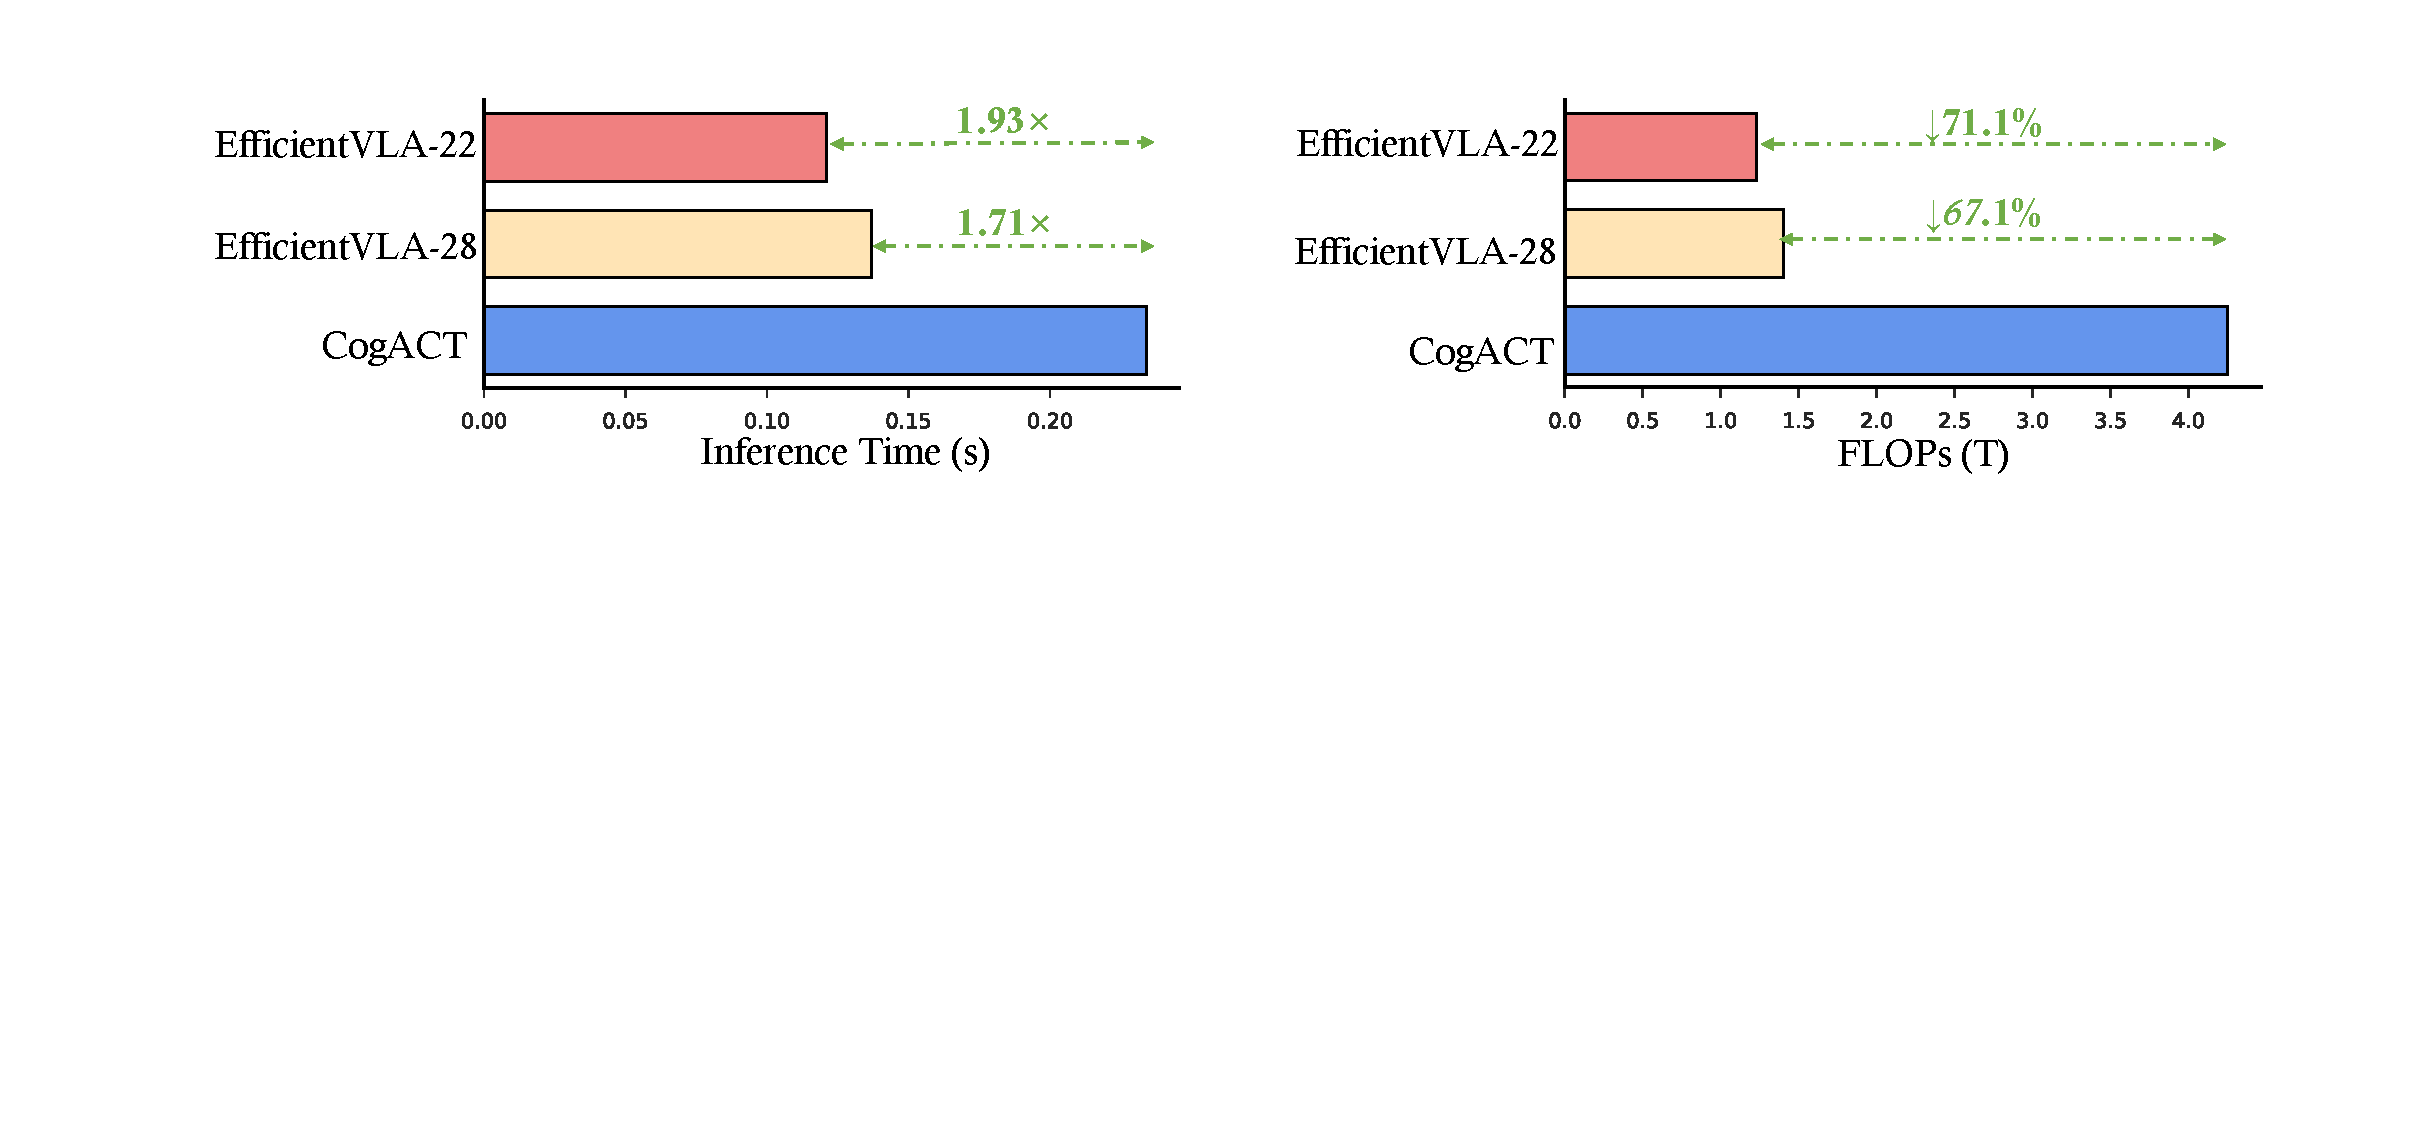
\includegraphics[width=0.99\linewidth]{figs/compare.pdf}
    \vspace{-5pt}
    \caption{\textbf{Efficiency analysis} in simulation, comparing FLOPs and inference time of our \mymethod{} variants against the original model backbone. \mymethod{}-22 and \mymethod{}-28 denote configurations retaining 22 and 28 LLM layers, respectively.}
    \label{fig:compare}
    \vspace{-10pt}
\end{figure}




\noindent \textbf{Scalability Evaluation}. Table~\ref{tab:scalability} illustrates the scalability of our proposed method across different sizes of the CogACT model. With the primary difference among the three models being the parameter size of their action modules, the results reveal that our method's effectiveness becomes more pronounced with larger models. Specifically, on the CogACT-Large model, our approach achieves a 2.0$\times$ inference speedup, while performance only marginally decreases from 76.7\% to 76.1\%. This increased impact is because action modules in larger models, having more parameters, inherently exhibit longer inference times, thus allowing our method to yield more significant accelerations. These findings also underscore the robustness of our method across models of various scales.


\noindent \textbf{Impact of Token Reduction Ratio and Cache Interval.} Table~\ref{table:token_cache} details our experiments on the \emph{pick coke can} task reveal distinct impacts of component-specific optimizations. Aggressively pruning visual tokens, down to retaining only 22\%, effectively lessens computational load for substantial, near-lossless acceleration. However, inference speed gains largely saturate beyond this point, with further token reduction yielding only marginal improvements, thereby revealing dominant system-level performance bottlenecks. Separately, for the diffusion-based action generator, we observed that increasing the cache reuse interval $N$ for intermediate attention and MLP features progressively and significantly accelerates action trajectory generation.






\begin{table}[!t] % 你也可以使用 [!htb] 来获得更灵活的放
  \caption{Performance impact of varying visual token reduction ratios (Left) and diffusion action head cache intervals (Right) as applied within our \mymethod{} framework.}
  \label{table:token_cache} 
  \begin{minipage}[c]{0.49\linewidth} % 第一个表格 minipage
    \centering
    \resizebox{\linewidth}{!}{ 
      \begin{tabular}{l|ccccc} % 第一列左对齐 (l)，其余列居中 (c)
        \toprule
        \textbf{Token} & 56 & 72 & 96 & 112 & 256 \\
        \textbf{Ratio} & 77.8\% & 71.8\% & 62.5\% & 56.2\% & 100.0\% \\ 
        \midrule
        \textbf{Accuracy} & 95.0\% & 95.3\% & 95.0\% & 96.0\% & 91.3\% \\
        \textbf{Inference time (s)} & 0.1866 & 0.1870 & 0.1889 & 0.1956 & 0.2342\\
        \textbf{FLOPs (T)} & 1.76 & 1.96 & 2.25 & 2.45 & 4.19\\
        \bottomrule
      \end{tabular}
    }
  \end{minipage}\hfill
  \begin{minipage}[c]{0.49\linewidth} 
    \centering
    \resizebox{\linewidth}{!}{
      \begin{tabular}{l|ccccc} % 第一列左对齐 (l)，其余列居中 (c)
        \toprule
        \textbf{Cache Interval} & 1 & 2 & 3 & 4 & 5 \\
        \midrule
        % 请确保 mylightyellow 和 mylightgreen 颜色已定义
        % \rowcolor{mylightyellow}
        \textbf{Accuracy} & 91.3\% & 94.0\% & 93.7\% & 90.3\% & 93.7\% \\
        % \rowcolor{mylightgreen}
        \textbf{Inference time (s)} & 0.2342 & 0.2031 & 0.1987 & 0.1953 & 0.1909 \\
        \textbf{FLOPs (T)} & 4.190 & 4.161 & 4.155 & 4.150 & 4.144\\
        \bottomrule
      \end{tabular}
    }
  \end{minipage}
\end{table}







\begin{table}[!t]
\begin{center}
    \setlength\tabcolsep{4pt} % 调整列间距
    \caption{\label{tab:ablation_model_compression} \textbf{Ablation study} on our \mymethod{}, where 'Layer' denotes applying only the LLM layer pruning component, and 'MLP' refers to a distinct strategy of compressing 25\% of MLP weights within each layer.}
    \resizebox{0.85\columnwidth}{!}{%
        \begin{tabular}{c|cccc|ccc}
        \toprule\toprule
        & \multicolumn{2}{c}{\textbf{Model Compression}} & \textbf{Visual Token} & \textbf{Action} & \textbf{Success} & \textbf{Inference}  & \textbf{Speedup$\uparrow$} \\
        \cmidrule(lr){2-3} % 为 model compression 的子列添加分隔线
        &  \textbf{Layer} & \textbf{MLP} & \textbf{Pruning} &\textbf{Cache} & \textbf{Rate}&\textbf{Time (s)} & \\
        \midrule\midrule
        % \rowcolor{lightlightlightred}
        Ex0 & \multicolumn{1}{c}{\textcolor{red}{\ding{55}}} & \textcolor{red}{\ding{55}} & \textcolor{red}{\ding{55}} & \textcolor{red}{\ding{55}} & 91.3\% & 0.2342 & 1.00$\times$ \\

        Ex1 & \multicolumn{1}{c}{\textcolor{red}{\ding{55}}} & \textcolor{red}{\ding{55}} & \textcolor{green}{\ding{51}} & \textcolor{red}{\ding{55}} & 95.6\% & 0.1866 & 1.25$\times$ \\

        Ex2 & \multicolumn{1}{c}{\textcolor{red}{\ding{55}}} & \textcolor{red}{\ding{55}} & \textcolor{red}{\ding{55}}& \textcolor{green}{\ding{51}}  & 93.7\% & 0.1909 & 1.23$\times$ \\
        
        % \rowcolor{lightlightlightyellow}
        Ex3 &\multicolumn{1}{c}{\textcolor{green}{\ding{51}}} & \textcolor{red}{\ding{55}} & \textcolor{green}{\ding{51}} & \textcolor{red}{\ding{55}} & 85.7\% & 0.1604  & 1.46$\times$ \\
        Ex4 &\multicolumn{1}{c}{\textcolor{green}{\ding{51}}} & \textcolor{green}{\ding{51}} & \textcolor{red}{\ding{55}} & \textcolor{red}{\ding{55}} & 92.3\% & 0.1638  & 1.43$\times$\\
        % \rowcolor{lightlightlightgreen}
        Ex5 &\multicolumn{1}{c}{\textcolor{green}{\ding{51}}} & \textcolor{green}{\ding{51}} & \textcolor{red}{\ding{55}} & \textcolor{green}{\ding{51}} & 93.3\% & 0.1387  & 1.69$\times$\\
        % \rowcolor{lightlightgreen}
        Ex6 &\multicolumn{1}{c}{\textcolor{red}{\ding{55}}} & \textcolor{red}{\ding{55}} & \textcolor{green}{\ding{51}} & \textcolor{green}{\ding{51}} & \textbf{95.3}\% & 0.1592 & 1.47$\times$ \\
        Ex7 &\multicolumn{1}{c}{\textcolor{green}{\ding{51}}} & \textcolor{green}{\ding{51}} & \textcolor{green}{\ding{51}} & \textcolor{green}{\ding{51}} & 93.3\% & \textbf{0.1213}  & \textbf{1.93$\times$} \\
        \bottomrule\bottomrule
        \end{tabular}
    }
\end{center}
\vspace{-2em}
\end{table}


\subsection{Ablation Study}

We conducted an ablation study on the components of our proposed framework, using the \emph{pick coke can} task as an illustrative example. As suggested by prior analysis (e.g., Figure~\ref{fig:bottleneck} (a), solely optimizing visual tokens for VLA inference tasks yields limited acceleration; retaining just 56 tokens resulted in a mere 1.23$\times$ speedup, although the success rate paradoxically rose from 91.3\% to 95.6\%. This underscores the inherent limitations of token-centric optimization methods, such as VLA-cache, and affirms that achieving substantial VLA inference acceleration viable for hardware deployment necessitates a more model-centric strategy. In contrast, our model compression approach—concurrently pruning layers and compressing MLP in the remaining layers—achieved a 1.43$\times$ speedup. Critically, when all components were integrated, a 1.93$\times$ speedup was realized, and the overall task success rate still saw an improvement of 2\% points. These collective results highlight the imperative and significance of adopting a structured framework for effective VLA inference acceleration.
